\subsubsection{Variante A: Alles Analog}
In dieser Variante wird möglichst alles via analoge Signalpfade geführt. So kann zum Beispiel die Signalverzögerung durch Allpass-Filter realisiert werden. Fokus ist auf Robustheit und Signalreinheit.
\begin{figure}[H]
	\centering
	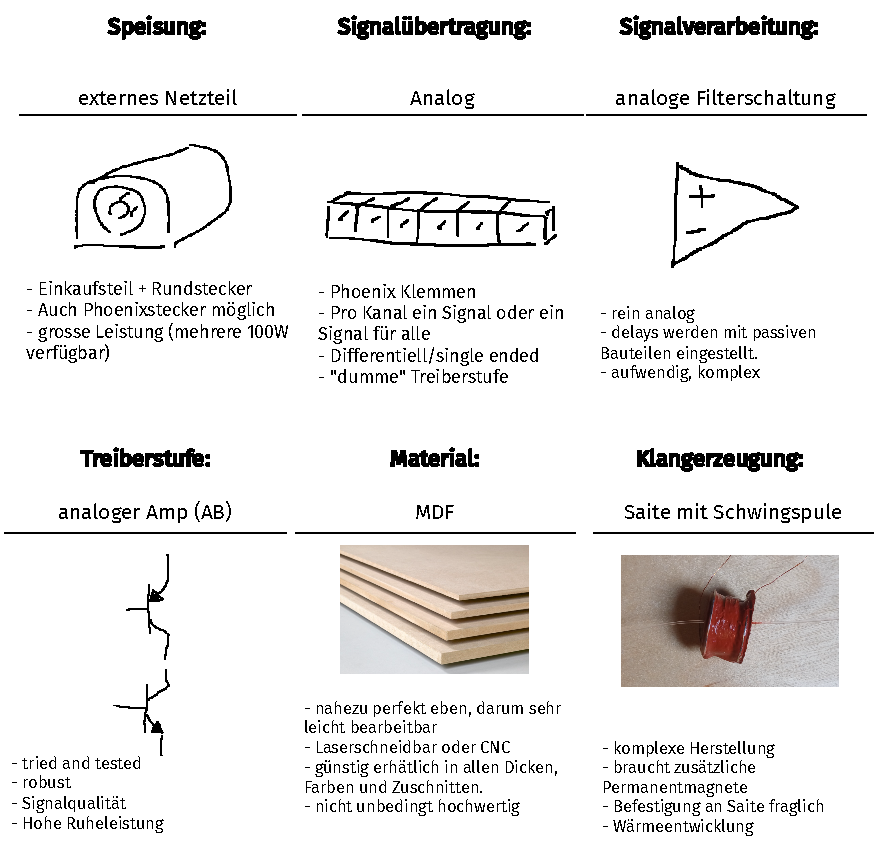
\includegraphics{pictures/VarianteA_allesAnalog.pdf}
	\caption{Variante A}
\end{figure}
\paragraph{Vorteile} Resultate sind relativ schnell messbar. Programmierarbeit erübrigt sich komplett. Zudem sind rein analoge Designs tendenziell robuster und langlebiger. Durch die fehlende Abtastung bleiben Höhenanteile erhalten und die Signalqualität eher hochwertiger.
\paragraph{Nachteile} Fehlersuche ist rein messtechnisch möglich. Nachträgliche Änderungen sehr teuer und Zeitaufwändig. Der Überwachung sind starke Grenzen gesetzt: So muss bei einem Unterbruch der gesamte Signalpfad durchgemessen werden. Ein weiterer Nachteil ist die nur schwer zu realisierende Skalierbarkeit.
\newpage
\paragraph{Risikoanalyse}
Durch sich bewegende Teile, welche unter Umständen durch den Benutzer berührt werden können entsteht zum einen ein Risiko einer leichten Verletzung. Zum anderen könnte die physikalische Montage von analoger Leistungselektronik auf MDF zu einer Brandgefahr führen. Zudem können sehr leicht durch fehlende, unsaubere oder falsche Steckverbindungen Funktionsfehler auftreten.
\begin{figure}[H]
	\centering
	\includegraphics[width=\textwidth*4/5]{pictures/risks-Variante A_ Alles analog.png}
	\caption{Risikoanalyse der Variante A}
\end{figure}
\newpage
\subsubsection{Variante B: Drahtlos \& Portabel}
Der Hauptfokus dieser Variante ist maximale mobilität und minimale Steckverbindungen. Dies wird zum einen durch ein Batterie erreicht, und zum anderen durch eine drahtlose Signalübertragung.
\begin{figure}[H]
	\centering
	\includegraphics{pictures/VarianteB_drahtlosPortabel.pdf}
	\caption{Variante B}
\end{figure}
\paragraph{Vorteile} Da hier die Datenübertragung ohne Stecker auskommt, kann hier im Einsatz komplett auf Kabel verzichtet werden. Somit vereinfachen sich insbesondere weiträumigere Setups, in dem das Gerät weiter weg aufgestellt ist. Als einziger Stecker bleibt ein Ladestecker für die Batterie übrig. Für die Einbindung von Batterien bzw. deren Ladezyklus gibt es zudem bereits sehr viele fertige Komponenten.
\paragraph{Nachteile} Die korrekte Implementierung des Signalpfades von Bluetooth oder Wifi über DSP, den DAC und die D-Klasse Endstufe wird wohl einiges an Aufwand brauchen, insbesondere bei zeitkritischen Anwendungen wie dieser. Zudem entsteht je nach Batterietyp eine Brandgefahr, die zwar durch das Plexiglas vermindert ist aber dennoch z.B. andere Materialien im Raum in Brand setzen kann.
\newpage
\paragraph{Risikoanalyse}
Zwar entfällt hier das Risiko einer falschen Steckverbindung komplett, jedoch erhöht sich durch die Anwesenheit einer Batterie die Brandgefahr deutlich. Dies auch wenn PMMA als Material verwendet wird, da sich die Batterie selbst schon entzünden kann. Zudem entsteht durch den komplexen Aufbau ein unter Umständen zeitintensive Designphase, welche auch mit HF-Layoutfehlern verbunden sein können.
\begin{figure}[h]
	\vspace{1cm}
	\centering
	\includegraphics[width=\textwidth*4/5]{pictures/risks-Variante B_ Portabel und Drahtlos.drawio.png}
	\caption{Risikoanalyse der Variante B}
\end{figure}
\newpage
\subsubsection{Variante C: High-End Audiophil}
Maximale Kontrolle steht bei dieser Variante im Zentrum. Nur bewährte und zuverlässige Komponenten sollen verwendet werden. Einkaufsteile sind nach Verzerrungsfreiheit und rauscharmen Signalpfaden auszuwählen. Preispunkt ist sekundär.
\begin{figure}[H]
	\centering
	\includegraphics{pictures/VarianteC_HighEndAudiophil.pdf}
	\caption{Variante C}
\end{figure}
\paragraph{Vorteile} Die Audioqualität als oberste Priorität begünstigt ein beeindruckendes Hörerlebnis. Zudem ist die Auswahl an bewährten Methoden und robusten Materialien ein Garant für eine lange Lebensdauer.
\paragraph{Nachteile} Als erstes ist hier sicher auch die Komplexität zu nennen, da sehr spezifische Bauteile ausgewählt werden müssen, die unter Umständen nicht weit verbreitet sind. Zum anderen wird hier auch das Budget sehr strapaziert, wohl über die Belastungsgrenzen hinaus.
\newpage
\paragraph{Risikoanalyse}
Die grosse Anzahl verschiedener eigens entworfenen Komponenten führt nebst der Gefahr eines \textit{Scope Creeps} auch eventuell zu Ungenauigkeiten oder unvorhergesehenen negativen Effekten. Zudem kommt zur Leistungselektronik der Endstufe auch die Leistungselektronik des Netzteils hinzu. Auch der Lautsprecher an sich kann überhitzen und zu Brandursachen führen.
\begin{figure}[H]
	\vspace{1cm}
	\centering
	\includegraphics[width=\textwidth*4/5]{pictures/risks-Variante C.png}
	\caption{Risikoanalyse der Variante C}
\end{figure}
\newpage
\subsubsection{Variante D: Einfache Anwendung, Plug'n'Play}
Möglichst einfache Anwendung ist zentral für ein überzeugendes Benutzererlebnis. Daher wurde diese Variante mit diesem Fokus generiert. Zudem ist ein Nebenfokus hier die günstige Herstellung des Systems.
\begin{figure}[H]
	\centering
	\includegraphics{pictures/VarianteD_EinfachPlugnPlay.pdf}
	\caption{Variante D}
\end{figure}
\paragraph{Vorteile} Da Datensignale und Speisung auf einem RJ45-Stecker geliefert werden, muss nur diese eine Verbindung hergestellt werden. Zudem ist mit dem MILAN-Protokoll eine automatische Bandbreitenreservation und somit keine Benutzerkonfiguration notwendig. Da DAC und Treiberstufe in einem Chip integriert ist, bleibt die Programmierung begrenzt. 
\paragraph{Nachteile} Da das Signal direkt vom PC generiert wird, muss dieses zuerst in das MILAN-Protokoll verpackt werden. Zudem muss ein AVB-fähiger Switch verwendet werden.
\newpage
\paragraph{Risikoanalyse}
Die Brandgefahr bleibt nach wie vor ein Hauptfaktor in der Risikoauswertung, bedingt durch die Verbindung von Holzfasern und Leistungsendstufen. Der noch nicht weitum verbreitete MILAN-Standard könnte hier auch zu Inkompatibilitäten, oder zumindest zu einem komplexen Setup führen. Auch könnte die Implementierung eines neuen Standards schnell \textit{Scope Creep} führen, da keine fix fertigen Lösungen bereitstehen.
\begin{figure}[H]
	\vspace{1cm}
	\centering
	\includegraphics[width=\textwidth*4/5]{pictures/risks-Variante D.png}
	\caption{Risikoanalyse der Variante D}
\end{figure}
\newpage
\subsubsection{Variante E: Neu ist besser}
Innovation und moderne Technologie ist das Hauptmerkmal dieser Variante. Es sollen möglichst die neusten Methoden und Komponenten verwendet werden. Etablierte Verfahren sind bereits vollumfänglich im Markt vorhanden und daher uninteressant. Daher werden alles entweder neue Technologien oder bislang nicht verwendete Ideen verwendet.
\begin{figure}[H]
	\centering
	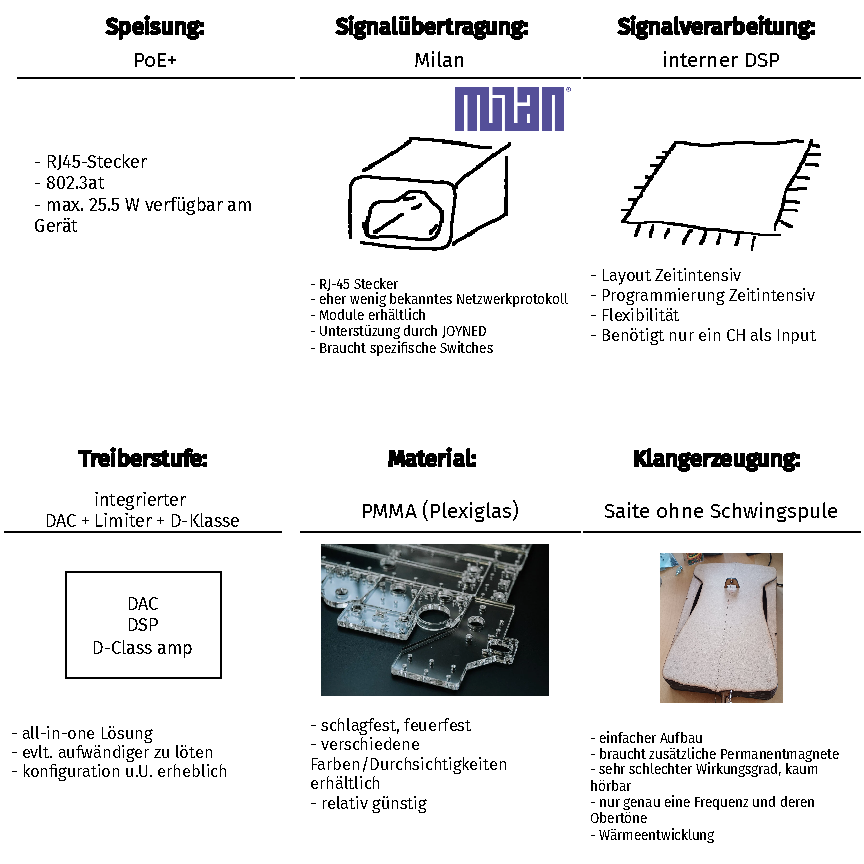
\includegraphics{pictures/VarianteE_Neuistbesser.pdf}
	\caption{Variante E}
\end{figure}
\paragraph{Vorteile} Durch die Neuheit und Innovation entsteht Freiheit: Es gibt in dem Sinne keine etablierte Verfahren oder Protokolle. Daher eröffnet sich ein Spielraum für Eigeninitiative.
\paragraph{Nachteile} Durch die undefinierten Variablen muss sehr viel Arbeit in deren Ausarbeitung investiert werden. So muss die gesamte Signalverarbeitung und die Kommunikation mit dem DAC definiert werden. Zudem entstehen unter Umständen weitere Kosten durch wenig verfügbare Bauteile.
\newpage
\paragraph{Risikoanalyse}
Nebst hohen Herstellungskosten kann hier eine stromdurchflossene Saite erhitzen und zu Verbrennungen führen. Des weiteren kann die Impedanz der Saite schlicht zu tief sein für die Endstufe, wodurch die Schwingung wenn überhaupt nur kaum wahrnehmbar also extrem leise erzeugt werden kann. Zudem entsteht durch den internen DSP auch hier die Gefahr des \textit{Scope Creep}, da die Signalverarbeitung potentiell recht umfangreich werden kann.
\begin{figure}[H]
	\vspace{1cm}
	\centering
	\includegraphics[width=\textwidth*4/5]{pictures/risks-Variante E.png}
	\caption{Risikoanalyse der Variante E}
\end{figure}
\newpage